In this chapter some experiments will be conducted. These experiments are modeled
after the scenarios described in the Theory chapter %TODO ref
The goal is to recreate these situation using the developed tool and running a
simulation with the described parameters. These simulations can then be used
to support or refute the assumptions that were made on how the diseases
theoretically should behave in those scenarios.

\section{Importance of $R_0$}
The role of the reproductive number $R_0$ was discussed in section \ref{sub:r0}.
It is the deciding factor for whether a disease is dying out ($R_0 < 1$) 
or able to live indefinitely ($R_0 > 1$). Calculating $R_0$ in complex social
networks is very hard because the structure of the networks has a big impact on $R_0$
in addition to the characteristics of the disease. For these experiments a very
rough estimation of $R_0=e_\mu \cdot p \cdot t_I$ is used as this is sufficient for estimating whether
the disease should die out in the experiment or life for a long time.
$e_\mu$ is the average amount of connection per node and $t_I$ the time it takes
for an infection to be cured, let $N$ be the total
amount of nodes in the network and $E$ the total amount of edges then
$e_\mu=\frac{E}{N}$. $p$ is the probability for a node to get infected
if one of its neighbors has the disease.

\subsection{The network}
\label{sub:exp_network}
The network that is used in these experiments contains 3 groups with 5000 nodes
each. Group 1 has 5 intra group connections for each node, group 2 has 4 and
group 3 has 3 intra group connections. Between each pair of groups there are
2 connections per node. The resulting network can be seen in figure \ref{fig:exp_r0_network}
It contains a total of 15,000 nodes.

\begin{figure}
    \centering
    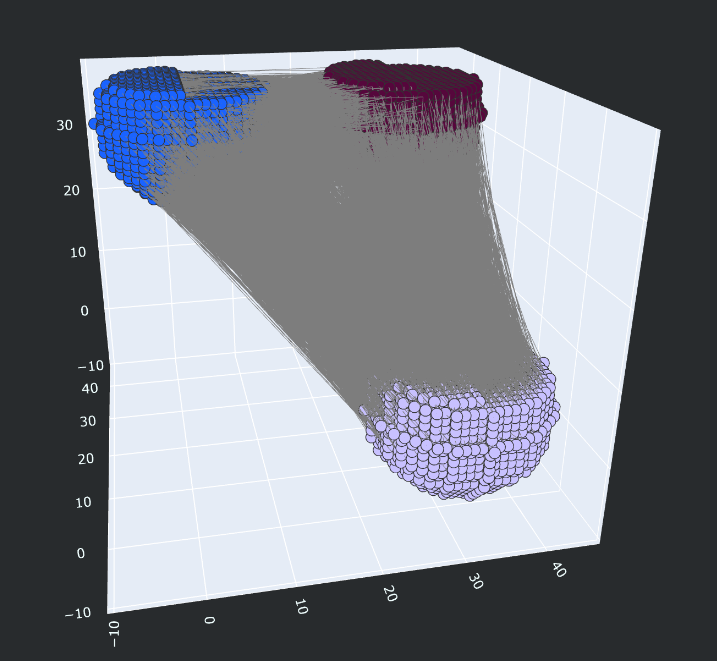
\includegraphics[width=0.5\linewidth]{images/experiment_r0_network.png}
    \caption{Structure of the network used for the $R_0$ experiments}
    \label{fig:exp_r0_network}
\end{figure}

Let $N_i$ be the amount of nodes in group $i$
then the amount of edges can be calculated using the following equation:
\begin{equation}
    E = \frac{n_1}{2} \cdot 5 + \frac{n_2}{2} \cdot 4 + \frac{n_3}{2} \cdot 3 + \frac{n_1+n_2}{2} \cdot 2 + \frac{n_1+n_3}{2} \cdot 2 + \frac{n_2+n_3}{2} \cdot 2
\end{equation}
Using that equation the it can be calculated that the network contains 60,000 edges.
This leads to an average amount of connections per node of $e\mu=\frac{60,000}{15,000} \cdot 2 = 8$.
But the different groups also need to be viewed in isolation. If the $R_0$ value within
one group of nodes is bigger than one, the disease is likely to never die out in that group
and the nodes of that group will constantly spread the disease to the other groups.
An example of this is shown in the next section.

\subsection{Experiment with $R_0 < 1$}
Since this experiment will use the same network as the one for a $R_0 > 1$ the
facor $e_\mu$ is static and cannot be changed. This makes $p$ the only deciding
factor for $R_0$ it can be calculated using $p = \frac{R_0}{e_\mu \cdot t_I}$ so in this case with $t_I=5$
with $R_0 < 1$, $p < \frac{1}{40}$. For cases with $R_0$ close to 1 there is still
a decent chance that the disease dies out even if $R_0 < 1$. $p=0.024$
is chosen for an estimated $R_0=0.96$ to ensure that the disease dies out in a finite
amount of steps.

The parameters for the disease of this experiment then are:
\begin{itemize}
    \item (vaccinated) fatality rate: 0
    \item (re-, vaccinated) infection rate: 0.024
    \item infection period $t_I$: 5
    \item initial infections: 5
    \item cure chance: 1
    \item immunity period: 0
    \item infectiousness factor: 1
\end{itemize}

Running the simulation shows that the disease is never able to spread to a large
amount of people and dies out after only \~9 steps. This can also be seen in the first graph
of figure \ref{fig:exp_r0_small}
which shows the amount of new infections per cycle. 
Increasing the initial amount of infected nodes to 5,000 shows that with
such a large amount of infections the disease still dies out after only \~20 steps

% is now able to spread to a lot of nodes intially.
% As the disease now has enough infected nodes to avoid dying out at random because of 
% randomness, it can be seen that it actually never dies out, as can be seen in the second graph
% of figure \ref{fig:exp_r0_small}. It constantly has between 50-100 new infections eveen though
% the estimated $R_0$ was only 0.96. This is due to the fact mentioned earlier, that each group
% also needs to be viewed in isolation: Group 1 has 9 connections per node so $R_0^1 = 0.02 * 7 * 5 = 1.08$
% which is bigger than 1. This means the disease has a chance to never die out within group 1 and is constantly
% spreading to the other groups from group 1.

Lowering $p$ to 0.02 results in an $R_0=0.9$ for group 1 and a total estimated $R_0=0.8$,
with these values the disease should die out in a finite amount of steps.
In this case it took \~40 steps for the disease to die out, the right graph of figure \ref{fig:exp_r0_small}
shows the amount of new infections up to that point.

\begin{figure*}
    \centering
    \begin{subfigure}[b]{0.475\textwidth}
        \centering
        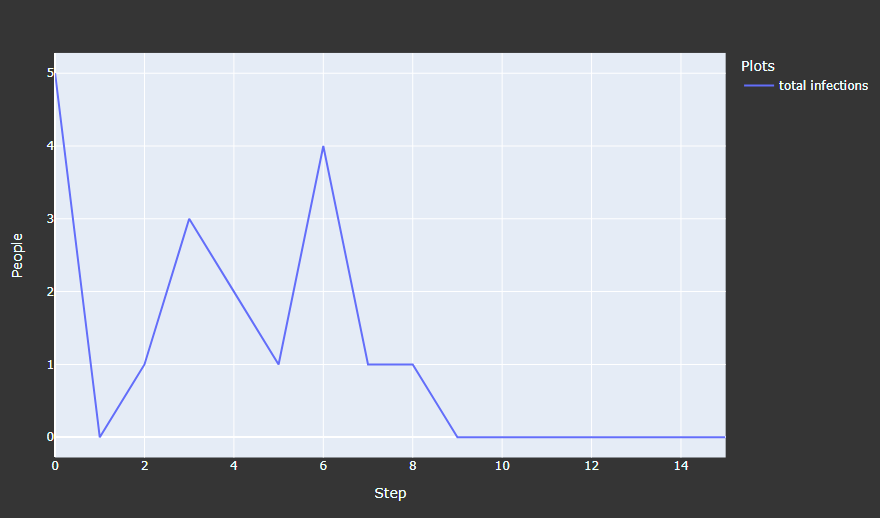
\includegraphics[width=\textwidth]{images/exp_r0_small_1.png}
        \caption[Network2]%
        {{\small Infection counts with 5 initial infections}}   
    \end{subfigure}
    \hfill
    \begin{subfigure}[b]{0.475\textwidth}  
        \centering 
        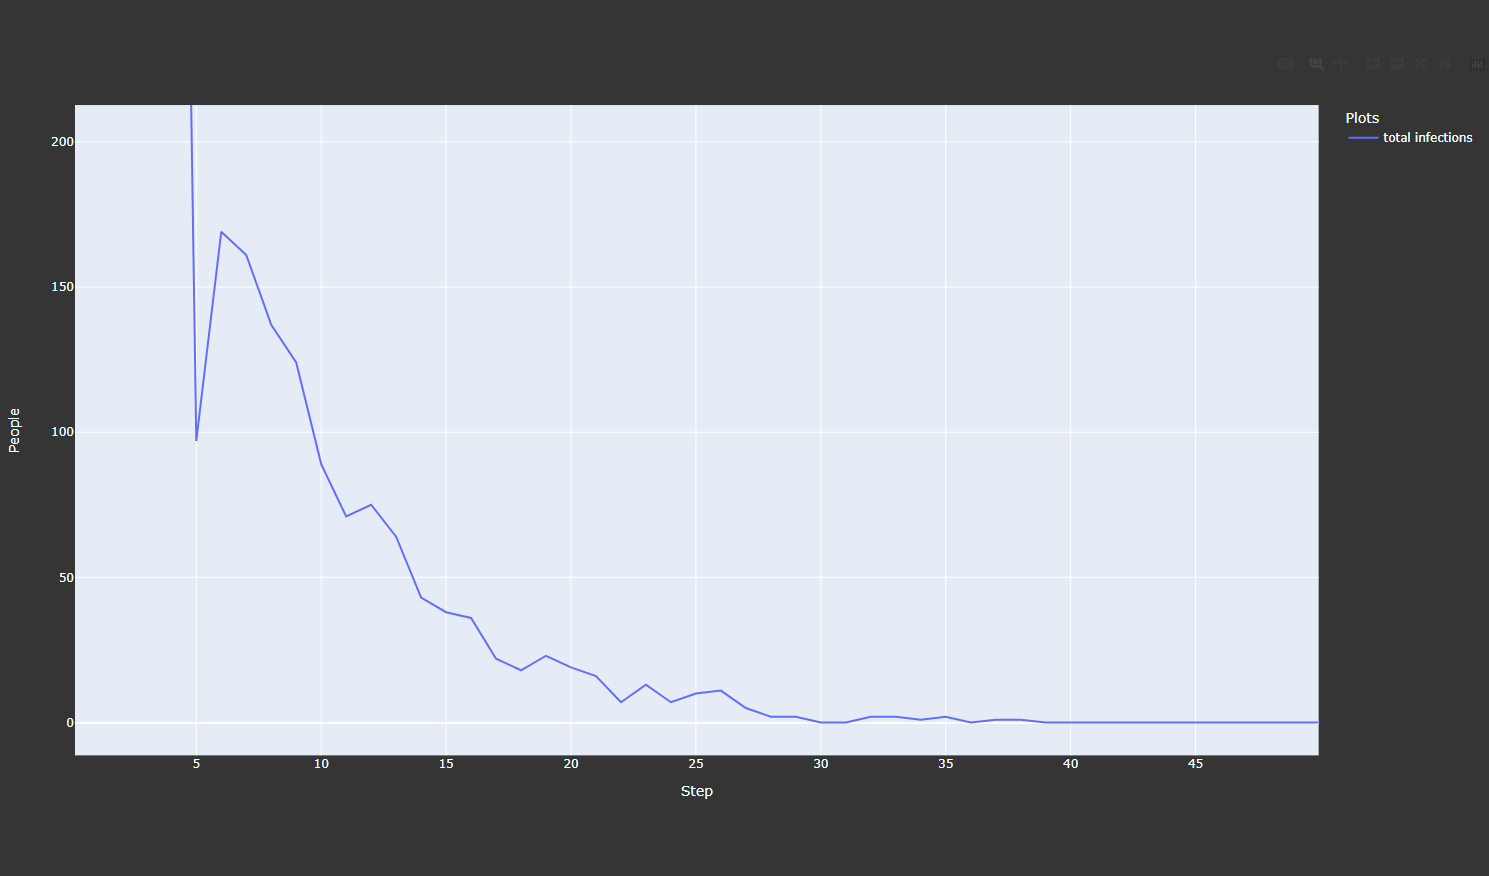
\includegraphics[width=\textwidth]{images/exp_r0_success.png}
        \caption[]%
        {{\small Infection counts with 5000 initial infections, showing that the disease
        still dies out after \~40 steps}}    
    \end{subfigure}
    \caption[ Experiment with an estimated $R_0$ of 0.96 and $p = 0.024$ ]
    {\small Experiment with an estimated $R_0$ of 0.96 and $p = 0.024$} 
    \label{fig:exp_r0_small}
\end{figure*}



This experiment supports the theory that for a $R_0 < 1$ the disease will die out
in a finite amount of steps. 

\subsection{Experiment with $R_0 > 1$}
This network uses the same network as the previous one, so $p$ is again the deciding
factor for $R_0$. $p = \frac{R_0}{e_\mu \cdot t_I}$ so for this case with $R_0 > 1$, $p > \frac{1}{40}$.
The theory created said that it should be sufficient to have a $p$
big enough to ensure $R_0 > 1$ in only one of the groups. Since group 1 has the most connections
$R_0^1 > 1$ if $p > \frac{1}{9\cdot5} = 0.0222$.
Since the closer $R_0$ to 1 the higher the chance the disease randomly dies out $p=0.03$ is chosen
resulting in a $R_0^1 = 1.35$ and $R_0 = 1.2$ where $R_0^1$ is big enough for the disease
to have a decent chance to survive indefinitely.

The properties that were changed from the previous experiment are:
\begin{itemize}
    \item (re-, vaccinated) infection rate: 0.04
    \item initial infections: 50
\end{itemize}

Running the simulation shows that the disease consistenly dies out at around 70 steps.
The left graph in figure \ref{fig:exp_r0_big} shows the infection counts. The expectation
was that the disease has a decent chance to survive but even after 20 tries it never
survived once. This can be explained by the network structure: the nodes in group 1
have 9 connections but 4 of those are "worth less" as the nodes it can spread to in the
other groups are not able to spread the disease to another 9 new nodes but only 7 or 8
depending on the group. This means that when calculating $R_0$ the nodes in group 1 can not
be considered to have 9 connections, somewhere around 8 would be more accurate. This makes
$R_0^1 = R_0 = 1.2$ which is not high enough wor a decent chance of indefinite survival.

Increasing $p$ to 0.036 is enough to make the disease live indefinitely with $R_0 = 1.44$.
After running the simulation for 20,000 cycles the disease is still alive and infecting
new nodes. This supports the theory that with a $R_0 > 1$ there is a probability $> 0$
that the disease never dies out. 


\begin{figure*}
    \centering
    \begin{subfigure}[b]{0.475\textwidth}
        \centering
        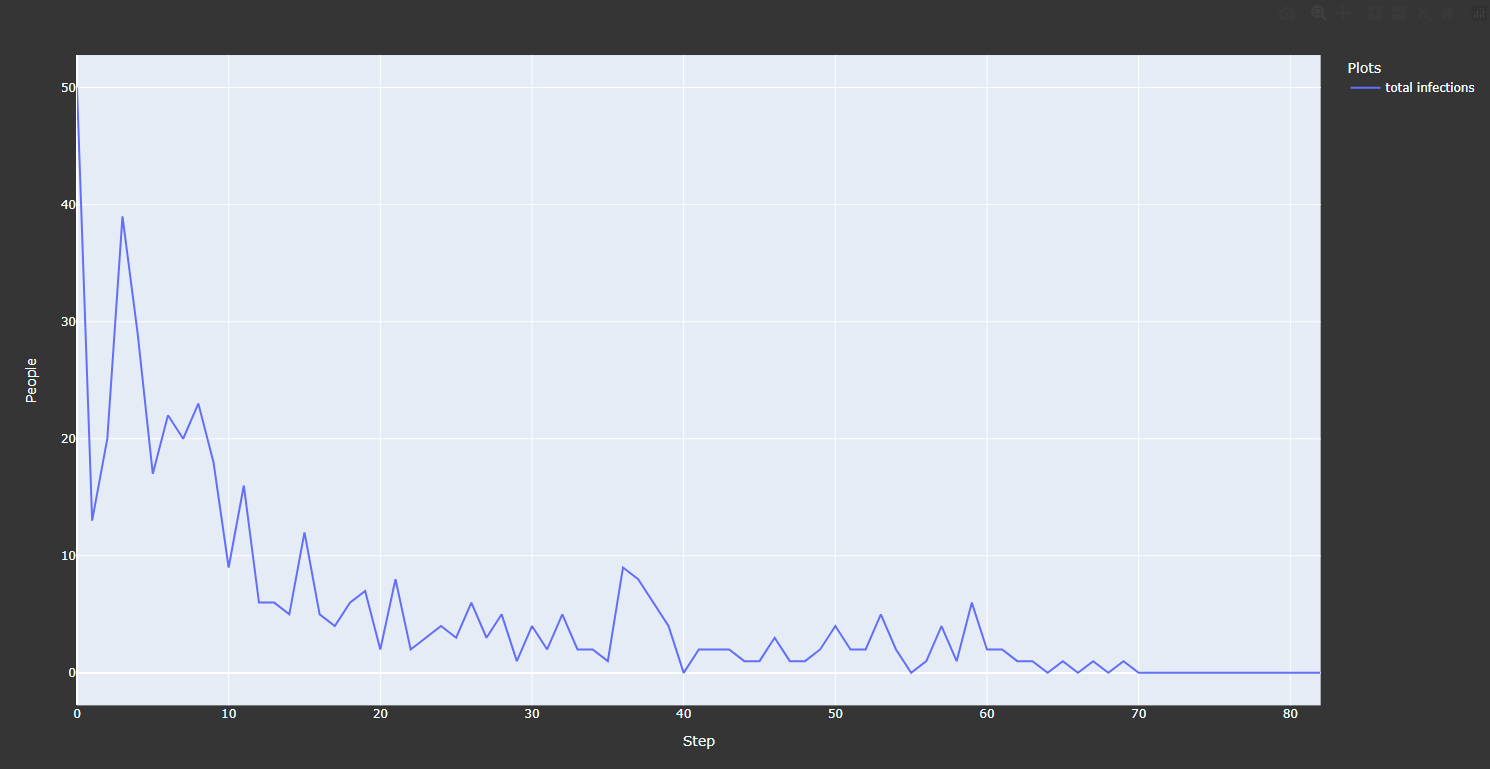
\includegraphics[width=\textwidth]{images/exp_big_r0_fail.png}
        \caption[Network2]%
        {{\small Infection counts with 50 initial infections and $p = 0.032$}}   
    \end{subfigure}
    \hfill
    \begin{subfigure}[b]{0.475\textwidth}  
        \centering 
        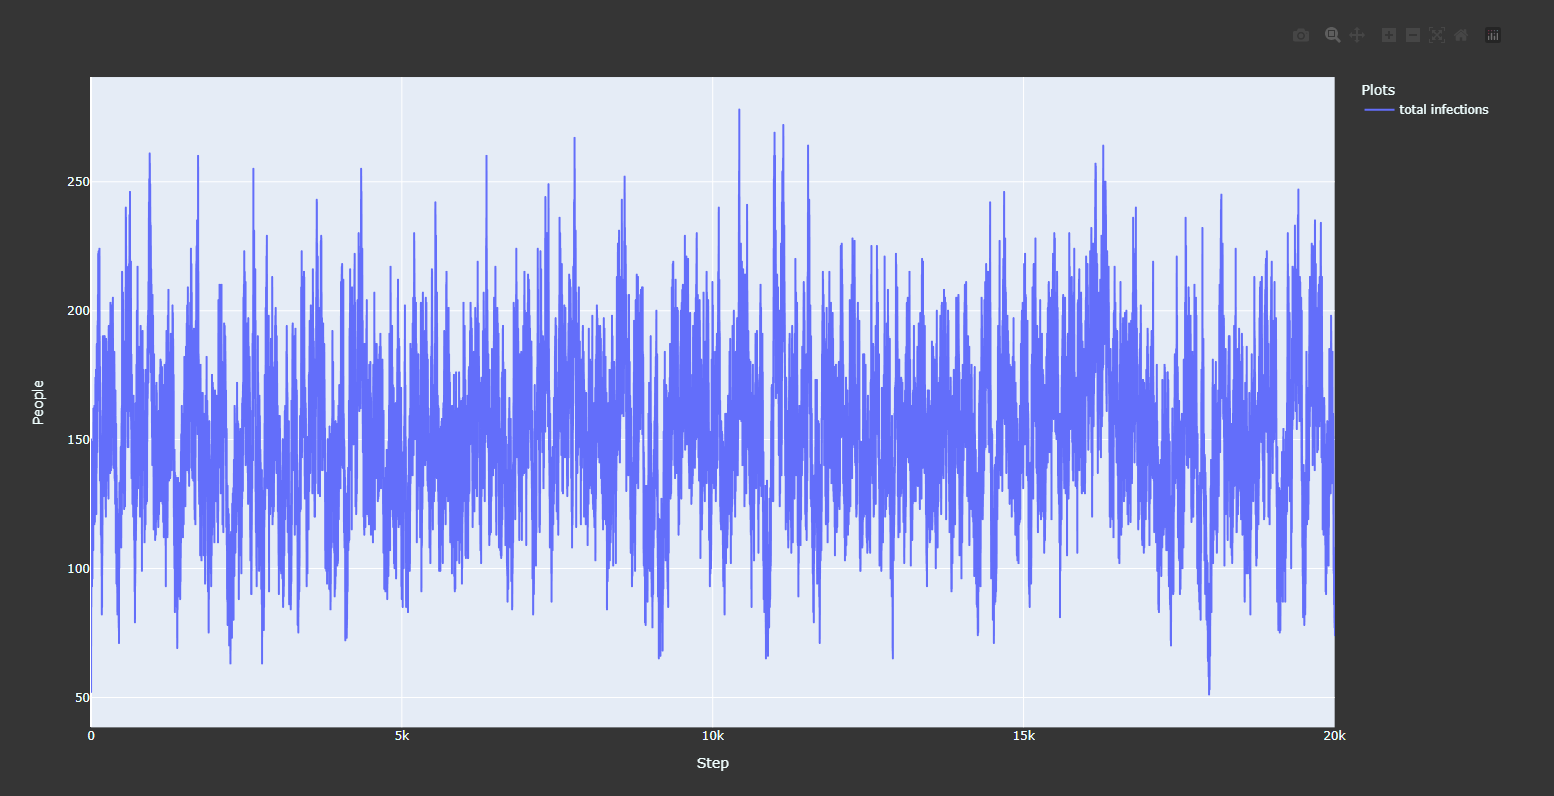
\includegraphics[width=\textwidth]{images/exp_big_r0_success.png}
        \caption[]%
        {{\small Infection counts with 150 initial infections and $p = 0.036$}}    
    \end{subfigure}
    \caption[Experiment with an estimated $R_0$ of 0.64 and $R_0^1 = 1.12$]
    {\small Experiment with an estimated $R_0$ of 0.64 and $R_0^1 = 1.12$} 
    \label{fig:exp_r0_big}
\end{figure*}

\subsubsection{Changing the network}
To show that the network structure indeed has an impact on $R_0$ this experiment
uses the same disease as the previous one with $p=0.036$ and 150 initial infections.
The network will have only half as many
edges, group 1 has 2 intra group connections for each node, group 2 has 2 and
group 3 has 2 intra group connections. Between each pair of groups there are
1 connections per node. This new network has 30,000 edges resulting in $e_\mu$ = 4.
Thus the new estimated $R_0=2\cdot0.375=0.75$ which is smaller than 1 so they
expectation is that the disease will die out even though it has the same infection 
rate as before.

After 20 cycles the disease has died out which supports the theory that the network structure
and thus $e_\mu$ has an impact on the spreading of diseases and the value $R_0$.
Graph \ref{fig:exp_change_network} shows the amount of infections until the disease died out.

\begin{figure}
    \centering
    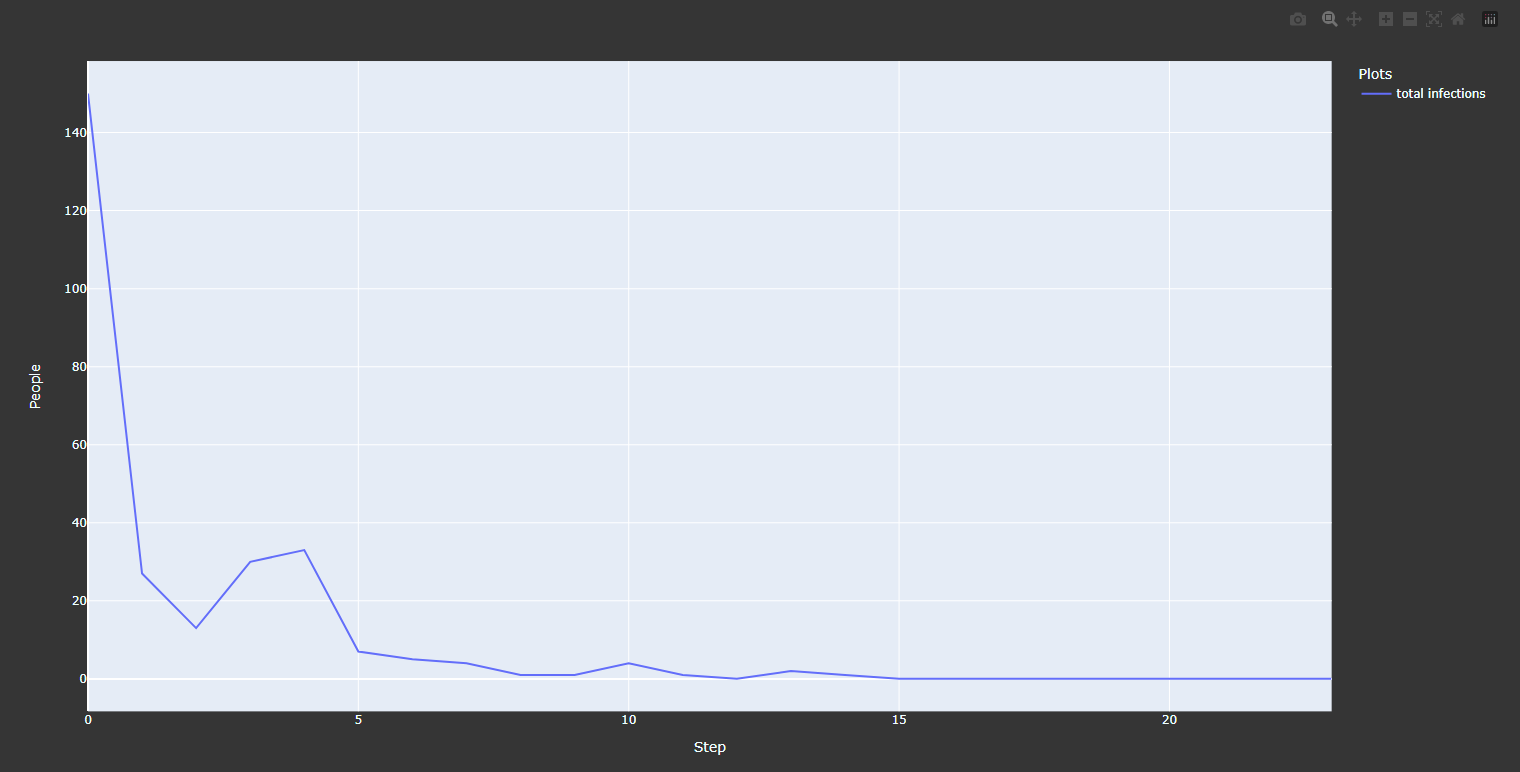
\includegraphics[width=0.5\linewidth]{images/exp_changed_network.png}
    \caption{Amount of infections with the same diseases ($p = 0.036$) but a network with half as many connections}
    \label{fig:exp_change_network}
\end{figure}

To support the theory from earlier that each group also needs to be viewed in isolation
when calculating $R_0$ the network is again changed. Group 1 has 8 intra group connections for each node,
group 2 has 1 and group 3 has 1 intra group connections. Between each pair of groups there are
2 connections per node which recuces $e_\mu$. The same $p = 0.036$ will be used resulting in $R_0 = 0.9$
while $R_0^1 = 1.44$. Running the simulation again it is shown that even though $R_0 < 1$ the
disease manages to survive indefinitely. But $R_0^1 = 1.44$ means the disease has a chance to never
die out within group 1 and is constantly spreading to the other groups from group 1. Figure
\ref{fig:exp_subgroups} shows the amount of infections per group. Group 1 has significantly more
infections and is keeping the disease alive, while group 2 and 3 have similar infection amounts.
This experiment shows how hard it is to estimate $R_0$
for complex networks, as the network might contain highly connected subgroups in which
the disease can live longer and spread to the rest of the network again.

\begin{figure}
    \centering
    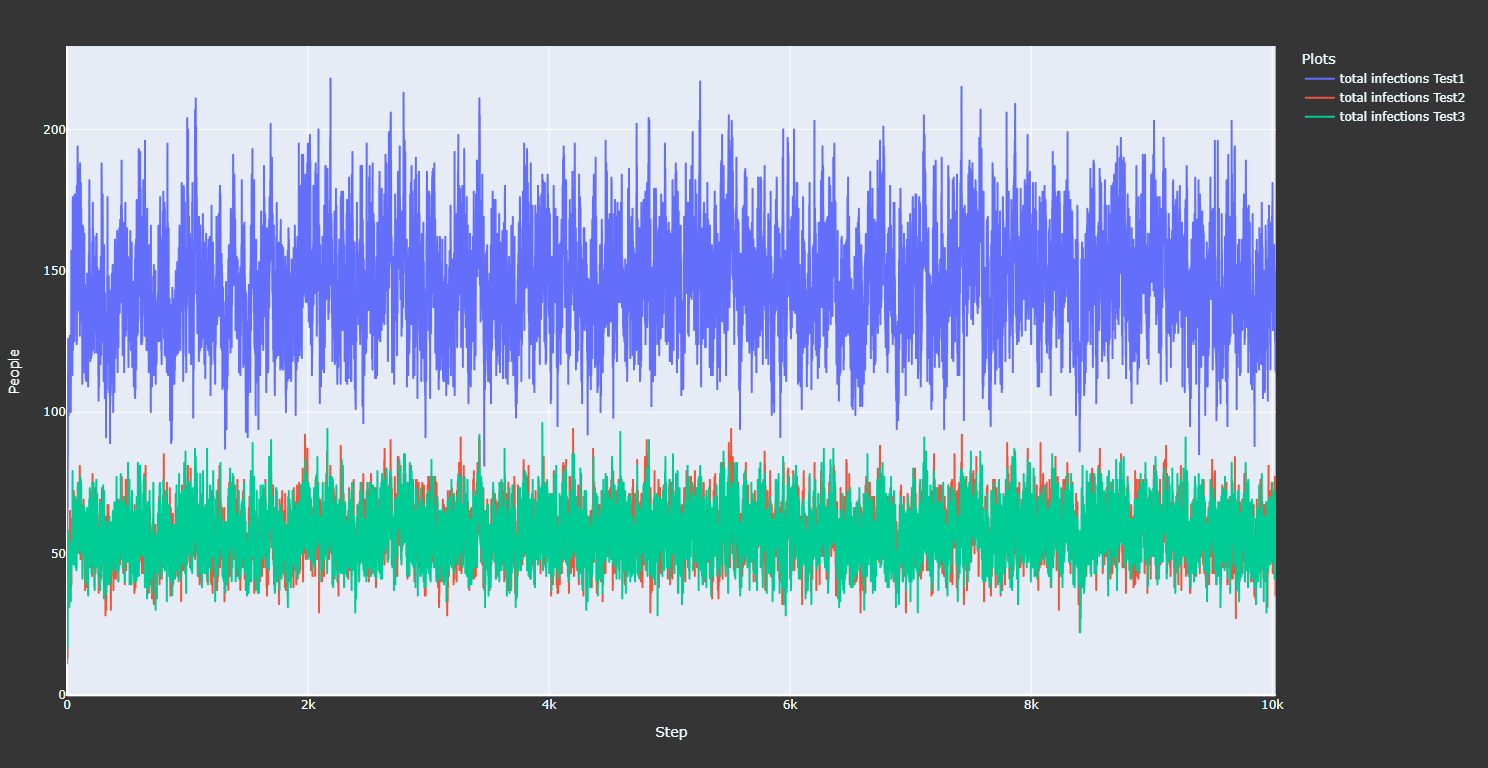
\includegraphics[width=0.5\linewidth]{images/exp_subgroups.png}
    \caption{Infections per group with $p = 0.036$ and $R_0 = 0.9$, the disease never dies out}
    \label{fig:exp_subgroups}
\end{figure}


\section{Multiple Diseases}
Interesting dynamics can be observed if multiple diseases are introduced into the same
social network. Cases with two diseases where one or both of the diseases have a $R_0 < 1$
do not make for an interesting scenario as once one disease has died out the problem just
gets reduced to one disease. But if both (or more) diseases have a $R_0 > 1$ then they 
will compete against each for survival, assuming a person can only be infected by one diseases
at a time, for example because they stay at home until they are cured so they can not get
infected by another disease during that period. Since a disease needs to constantly infect
new nodes to stay alive the diseases can rot other diseases out by infecting all nodes themselfes
thus leaving no availabe nodes to infect for other diseases.

For diseases with a similar $R_0$ the two diseases will each have \~50\% of infections.
Now consider a case where one diseases $d_1$ has $R_0^1=2$ and the second $d_2$ has $R_0^2=5$.
When the diseases are viewed in isolation theoretically both are able to survive as both
$R_0^1 > 1, R_0^2>1$. Looking at the situation where both diseases are in the same network,
$d_2$ will infect significantly more people than $d_1$, about 2.5 times as many. This means
that $d_2$ will have $~\frac{5}{7}$ of total infections during the first wave. As $d_2$ has
way more infected nodes during the first wave that makes it even easier for it to spread than
$d_1$. At the borders where susceptible nodes have connections to nodes infected with $d_1$
and also to nodes infected with $d_2$, $d_2$ will infect $\frac{5}{7}$ of those nodes. This
will slowly reduce the amount of nodes infected with $d_1$ until none are left and $d_1$ has died
out even though its $R_0^1>1$. This means in networks with more than one disease the one 
with the highest $R_0$ value is the one most likely to survive.

\subsection{Experiment}
This theory can again be supported by conducting an experiment using the developed simulation
tool. The network will be the same used in the previous experiment, consisting of 3 groups with
more intra group connections than inter group connections. The exact structure is explained
in section \ref{sub:exp_network}.

Two diseases are used for this simulation:
\begin{itemize}
    \item %TODO
\end{itemize}

First the experiment is run with the two diseases separately to show that they never die out
on their own. The results can be seen in figure \ref{fig:exp_multiple_diseases_individual}
which shows the amount of new infections until cycle 5000 indicating that the individual 
diseases have not died out until then.

\begin{figure*}
    \centering
    \begin{subfigure}[b]{0.475\textwidth}
        \centering
        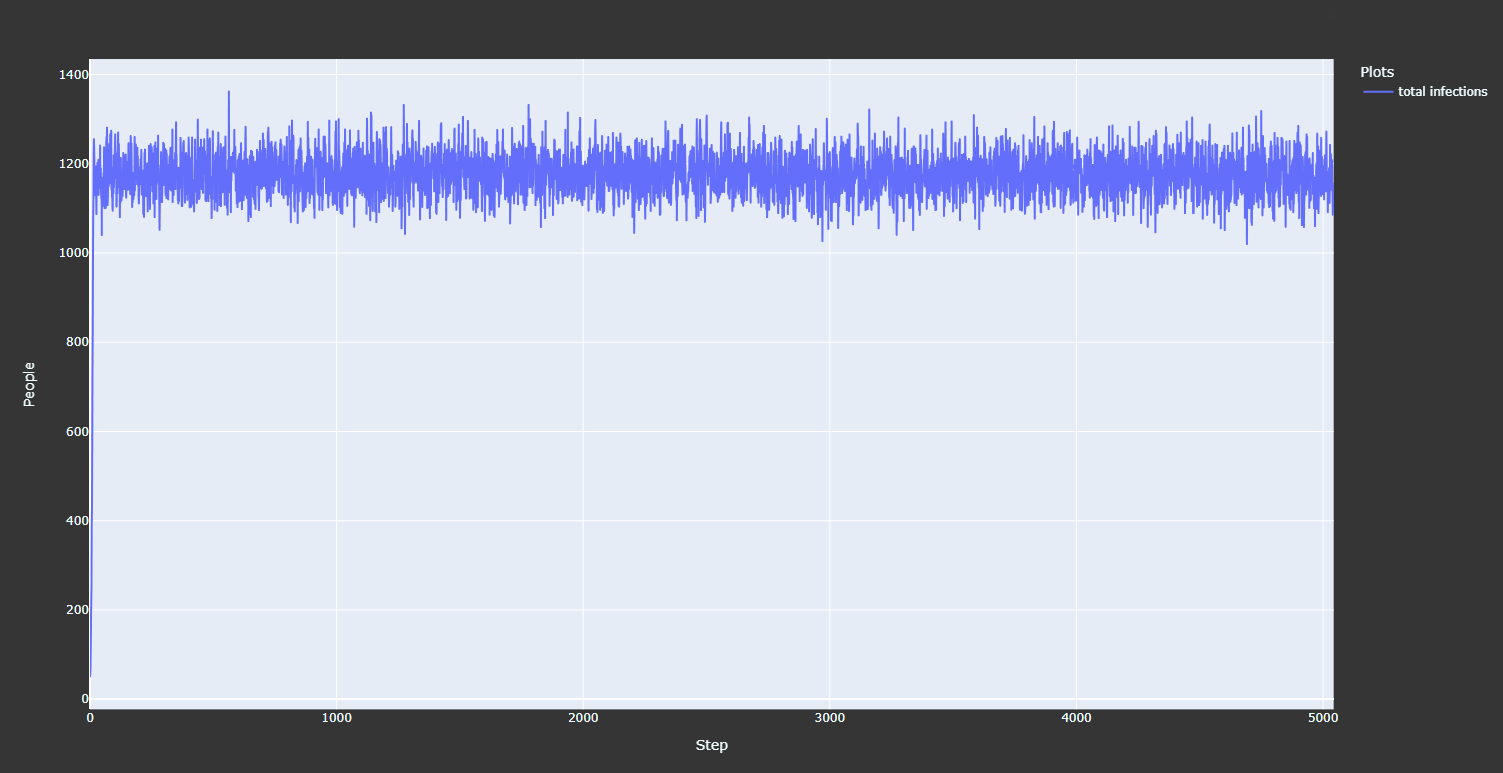
\includegraphics[width=\textwidth]{images/exp_multiple_diseases_d1.png}
        \caption[Network2]%
        {{\small Infection counts for disease 1 with 50 initial infections and $p = 0.06$}}   
    \end{subfigure}
    \hfill
    \begin{subfigure}[b]{0.475\textwidth}  
        \centering 
        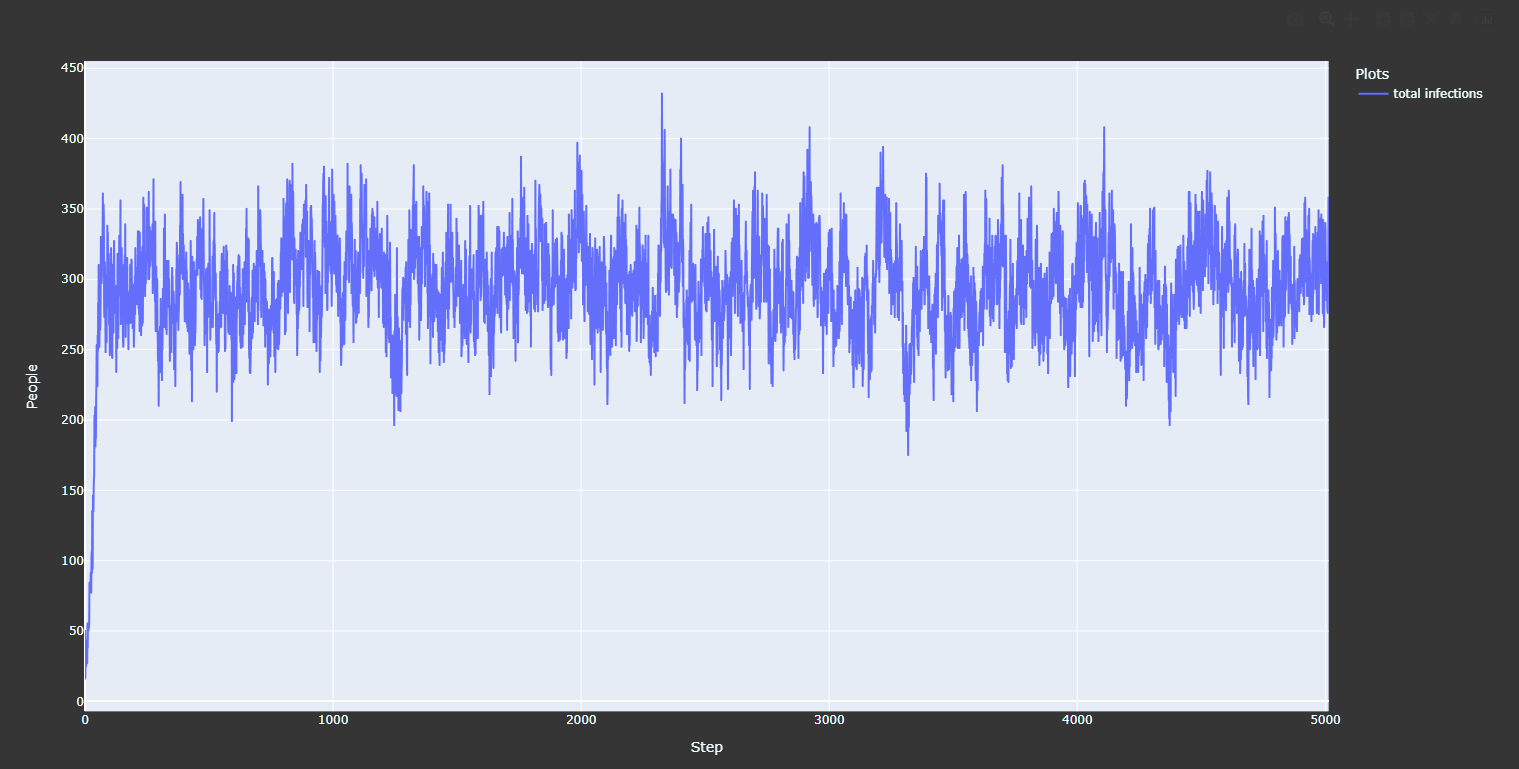
\includegraphics[width=\textwidth]{images/exp_multiple_diseases_d2.png}
        \caption[]%
        {{\small Infection counts for disease 2 with 150 initial infections and $p = 0.04$}}    
    \end{subfigure}
    \caption[Experiment to show both diseases never die out on their own]
    {\small Experiment to show both diseases never die out on their own} 
    \label{fig:exp_multiple_diseases_individual}
\end{figure*}

Now both diseseases are used at the same time. After 40 cycles
$d_2$ has died out because the new infections of $d_1$ have increased so much that
not enough nodes are availabe for $d_2$ to infect. This increase in infections with $d_1$ and
decrease in infections with $d_2$ is shown in figure \ref{fig:exp_multiple_diseases}.

\begin{figure}
    \centering
    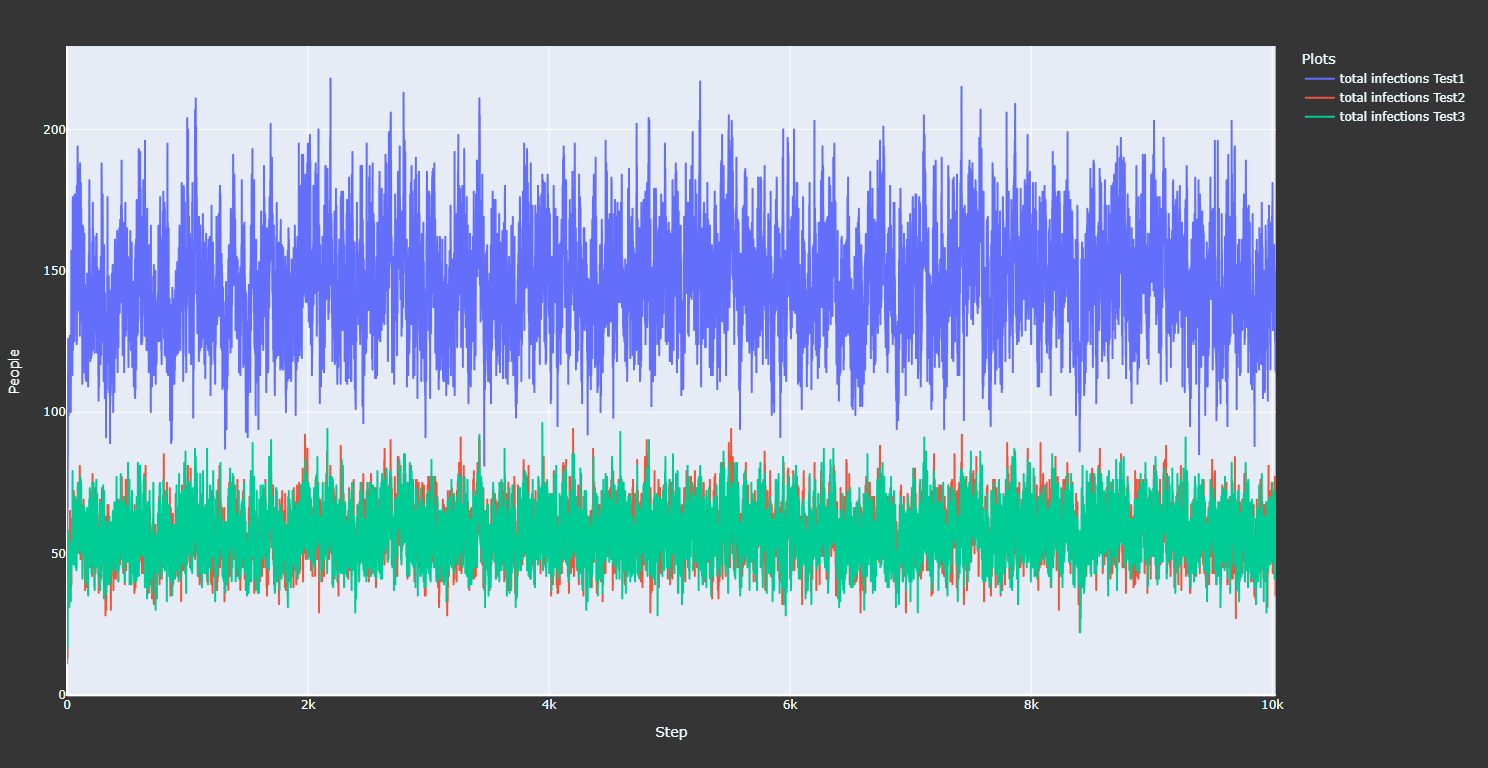
\includegraphics[width=0.5\linewidth]{images/exp_subgroups.png}
    \caption{Infections per disease with $p = 0.06$ and $p = 0.04$, disease 2 dies out after 40 steps even though it did not die out when the two diseases were simulated in isolation}
    \label{fig:exp_multiple_diseases}
\end{figure}

This supports the theory that in networks with multiple highly infectious diseases the
one with the highest $R_0$ value is the one most likely to survive.

\section{Small-World Phenomenon}
The small-world phenomenon is also known as six degrees of separation. The theory is that
in an arbitratily large social network the length of the path from one person to any other
person is on average only 6 steps long. To support this theory Stanley Milgram conducted
an experiment in the 1960s \cite{smallWorld}. In this experiment Milgram gave a letter to 
a random source person in Nebraska (US) and told them to deliver it to a target person in
Massachusetts (US). The source person was only given basic information about the target like 
address and occupation and each person was only allowed to send the letter to someone they
knew on a first name basis with the goal to get the letter closer to its target. Any person
in this chain was given the same information. After many iteration of this experiment the 
average amount of persons it took to deliver the letter to its target was between 5 and 6 persons
leading to the name of the six degrees of separation principle.

This experiment does not always find the shortest path though as the people forward the letter
only to the person they assume to be closest to the target. Unkownst to them there might
be another person they know who is much closer to the target making for a shorter path which
is never discovered. To find the true shortest path each participant would have to forward
the letter to all their friends while keeping track of which path the letter has taken.
Then after all letters have arrived at the target the true shortest path is the one of the
letter that needed the least amount of persons to arrive.

\subsection{Experiment}
For this experiment a network with only one group is created. That group
contains 10,000 nodes with each node having 6
connections. Though this network is not totally accurate to a real situation. Usually 
a friends network of a person is tightly coupled, the friends of a person usually also know
each other and their friends know the initial person etc. Also a person mostly knows
others that live in an area close to them and only fewer persons that live farther away.
This leads to a highly connected network with only short connections and a few random longer connections.
The network used for this experiment uses only random edges which does not represent this
fact that the geolocically closer people are the more connections they have. However in the
current day the internet allows for way more connections over long distances which makes
the used network more valid in that context.

\begin{figure}
    \centering
    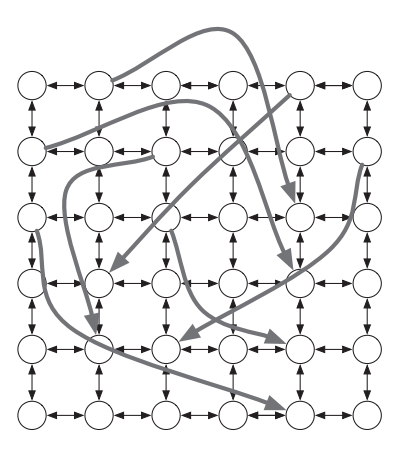
\includegraphics[width=0.5\linewidth]{images/sw_true_network.png}
    \caption{True structure of a network showing the friends of persons. The
    geolocically closer people are the higher the amount of connections. There
    are only few connections over longer range. (source: \cite{networks})}
    \label{fig:oscillation}
\end{figure}


To show that each node can be reached in only six steps, a disease with an infection rate
of 1 and infection duration of 1000 is used. Initially only one
node is infected. Figure \ref{fig:small_world_network} shows the network after 6 cycles.

\begin{figure}
    \centering
    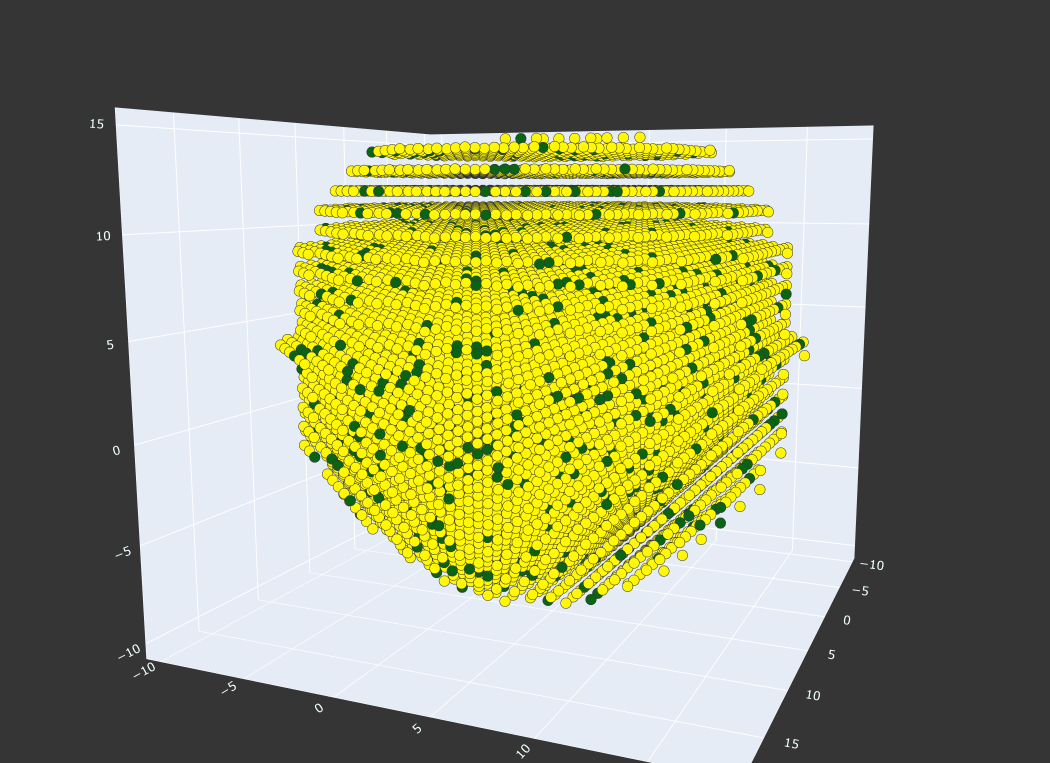
\includegraphics[width=0.5\linewidth]{images/small_world_network.png}
    \caption{Network after 6 cycles, yellow nodes have a shortest connection with 6 or less steps to the starting node,
    green ones have a shotest connection with more than 6 edges to the starting node}
    \label{fig:small_world_network}
\end{figure}

After cycle 7 all nodes are infected which means they were all able to be reached from the 
starting node in a maximum of 7 steps. The exact amounts of new infections per step are:
6, 30, 150, 717, 2893, 5306 and 897. Using these values the average shortest path length
can be calculated, it is \~5.5964. This coincides with the findings of Milgram \cite{smallWorld}
whose experiments showed the average length is somewhere between 5 and 6.

To reduce the limitation of the used network in regards to the random connections another
network structure could be used. This one closer models the existance of highly coupled
local friend groups where everyone knows each other and a few random connections to people
from other friend groups who are further away. This network uses a high amount of
groups with relatively few members each. In this case 100 groups of 5-10 people are used
where each node is connected to 4 others of the same group and each group of people is
connected to 3-4 other groups with only 0-1 edges per node. This again results in a network
where on average each node has 6 connections.

The same disease is used in this network and the state of the network after cycle 6
can be seen in figure \ref{fig:small_world_groups}.

\begin{figure}
    \centering
    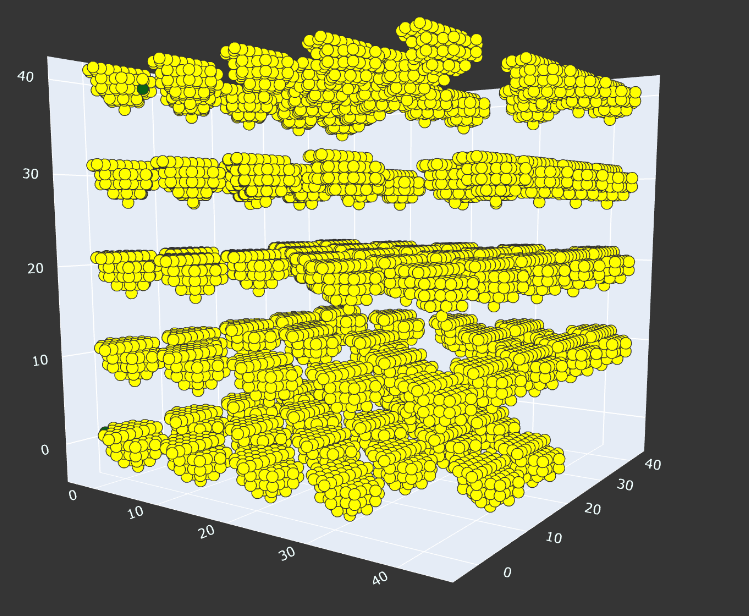
\includegraphics[width=0.5\linewidth]{images/small_world_groups.png}
    \caption{Network after 6 cycles, yellow nodes have a shortest connection with 6 or less steps to the starting node,
    green ones have a shotest connection with more than 6 edges to the starting node}
    \label{fig:small_world_groups}
\end{figure}

This shows that in this network it is also possible to reach all other nodes in only six steps,
even though there are only a few long distance connections and a lot of thightly coupled
small groups. The average path length in this experiment was \~5.6621


